\documentclass[letterpaper,12pt]{article}

\makeatletter
\newcommand{\raisemath}[1]{\mathpalette{\raisem@th{#1}}}
\newcommand{\raisem@th}[3]{\raisebox{#1}{$#2#3$}}
\makeatother
\newcommand{\tolstrut}{%
  \vrule height\dimexpr\fontcharht\font`\A+.1ex\relax width 0pt\relax
}

\DeclareRobustCommand{\textoverline}[1]{%
  \ensuremath{\overline{\mbox{\tolstrut#1}}}%
}
\newcommand{\overbar}[1]{\mkern 1.5mu\overline{\mkern-1.5mu#1\mkern-1.5mu}\mkern 1.5mu}
% csm-thesis automatically includes the following packages:
%% float
%% setspace
%% geometry
%% graphics
%% textcase
%% subfig

% Note: Two package options exist for your convenience: ``insane'' and ``nolabel''.  To use these options together separate them by a comma, ie. \usepackage[insane,nolabel]{csm-thesis}
% * \usepackage[insane]{csm-thesis}
% Turn off all document sanity checks.  This option can be used to render a ``sub-document'' that is part of the root thesis document.  It is important to note that you should NEVER disable this check on your root thesis document, as important format errors and warnings will be disabled.
% * \usepackage[nolabel]{csm-thesis}
% Disables automatic reference ``labeling'' of figures and tables.  By default the thesis template prepends any reference to a figure or table with ``Figure~'' or ``Table~''.  This option is meant for disabling the labeling behavior when a document already has the appropriate labeling.  It is important to note that if your document DOES NOT have the appropriate labeling (the reference label must EXACTLY MATCH the caption label) then it will not pass the format review.
\usepackage{csm-thesis}
\usepackage{ulem}
\newcommand{\dispdot}[2][.2ex]{\dot{\raisebox{0pt}[\dimexpr\height+#1][\depth]{$#2$}}}% \dispdot[<displace>]{<stuff>}
\newcommand\mtilde{\stackrel{\sim}{\smash{Q}\rule{0pt}{1.6ex}}}
% For inserting large multi-page tables:
\usepackage{array}
\usepackage{longtable}
\usepackage{amssymb}
\usepackage[mathscr]{euscript}
\usepackage{gensymb}
\usepackage[lite]{mtpro2}
\usepackage{bm}
\DeclareMathAlphabet      {\mathbfit}{OML}{cmm}{b}{it}
\DeclareFontFamily{OT1}{pzc}{}
\DeclareFontShape{OT1}{pzc}{m}{it}{<-> s * [1.10] pzcmi7t}{}
\DeclareMathAlphabet{\mathpzc}{OT1}{pzc}{m}{it}
% For inserting sideways tables and figures
\usepackage{graphicx}
\usepackage{rotating}
%\usepackage{caption}
%\usepackage{subcaption}





% Since hyperref and cite don't completely get along, the template now recommends using natbib:
% For an explanation, see http://www.tex.ac.uk/cgi-bin/texfaq2html?label=citesort
\usepackage[numbers]{natbib}
% If you wish to use ``cite'' instead then your choices are:
% 1) Don't use the hyperref package
% 2) Put ``cite'' before hyperref, resulting in no citation hyperlinks
% 3) Put ``cite'' after hyperref, resulting in ugly looking citations

% If you choose not to use natbib then you can set the standard ``numeric'' style like so:
%\bibliographystyle{unsrt}

% Important Note: math-mode in sections, titles, and other bookmarks will generate warnings with hyperref.  You can work around this by either:
% 1) Not using the hyperref package
% 2) Using \texorpdfstring{TeX Code}{PDF Replacement} to display an alternative bookmark (for example, \texorpdfstring{H$_2$O}{Water}).
% The thesis template will automatically import your document information into hyperref, so if you go to ``File | Properties'' in Adobe Acrobat it will display the title and author.  If you would like to over-ride this option then just change the line below to ``\usepackage[]{hyperref}''.
\usepackage{hyperref}

% For inserting programming code:
\usepackage{listings}

% For inserting landscape-mode objects:
\usepackage{pdflscape} % use ``lscape'' if you are not creating a PDF output

% For matrices:
\usepackage{amsmath}
\newcommand{\ii}{\textit{\i}}

\begin{document}
\chapter{Validation and Verification}
For the purposes of this thesis, the term ``verification" refers to code-to-code, and code-to-analytical results comparison. ``Validation" refers to code-to-experiment. The purpose of verification is to prove that a code is capable of accurately modeling the same physics. This step is usually taken before validation because there are sometimes cases where the code can match a set of experimental data but still not work for a more general case. The verification process is a crucial step to ensuring that the code performs as expected for a rigorous set of test cases. 

This chapter will consider a mixture of analytical and numerical verification test cases. A validation case for a wind turbine blade will also be examined. The purpose of these test cases is to ensure that BeamDyn is capable of performing as expected for beams with anisotropic material properties, complex geometry, and nonlinear displacements. The efficacy of the spectral element method as applied to GEBT will also be examined.

\subsection{Test Case 1 - Static bending of cantilever beam}
The first test case is a static analysis of an isotropic cantilever beam with a point moment applied at the tip of the beam as shown in \ref{fig:Case1}. This is a common benchmark problem that was first proposed by Simo \cite{Simo1985} and was also demonstrated in Wang et al.\ \cite{Wang:GEBT2014}. This problem demonstrates the ability of BeamDyn to analyze an isotropic beam with no initial curvature, and with highly nonlinear deflections. In fact, the displacement is so large that it the beam bends into a circular shape. The beam is discretized by two 5\textsuperscript{th}-order elements (i.e. the spectral order, $p=5$) with a beam total length of 10 inches along $x_1$. The material properties, $C^*$, are shown below. 
 \csmfigure{Case1}{figures/Case1}{4in} {Configuration for 10 inch beam.}
 
 \begin{align*}
 C^* = 10^3 \times
 	\label{tab:Stiffness 1}
 	{\left[\begin{matrix}
 		1770 & 0    & 0    & 0    & 0    & 0   \\
 		0    & 1770 & 0    & 0    & 0    & 0   \\
 		0    & 0    & 1770 & 0    & 0    & 0   \\
 		0    & 0    & 0    & 8.16 & 0    & 0   \\
 		0    & 0    & 0    & 0    & 86.9 & 0   \\
 		0    & 0    & 0    & 0    & 0    & 215
 	\end{matrix}\right]}
 \end{align*} 
which has units of $C^*_{ij}$ (lb), $C^*_{i,j+3}$(lb.in), and $C^*_{i+3, j+3}$(lb.in\textsuperscript{2}) for $i=1, 2, 3$. It is noted that the asterisk implies that sectional properties are resolved in the material basis, and the stiffness matrix in the inertial frame is given by $\uuline{C} = (\uuline{R}\,\uuline{R}_{\raisemath{6pt}{0}})\uuline{C}^*(\uuline{R}\,\uuline{R}_{\raisemath{6pt}{0}})^T$.


The analytical displacement in the $x_1$ and $x_3$ ($u_1$ and $u_3$ respectively), are calculated. The analytical displacements for this beam are given by Mayo \cite{Mayo-etal:2004}:

\begin{equation}
\label{eq: 5.1}
u_1 = \rho\;\text{sin}\bigg(\dfrac{x_1}{\rho}\bigg)-x_1; \quad u_3 = \rho\;\bigg(1-\text{cos}\bigg(\frac{x_1}{\rho}\bigg)\bigg)
\end{equation}
where,

\begin{equation}
\label{eq: 5.2}
\rho = \dfrac{EI_2}{M_{x2}}
\end{equation} 
The moment about $x_2$, $M_{x2}$, is given by

\begin{equation}
\label{eq: 5.3}
M_{x2}={\lambda\bar{M}_{x2}}
\end{equation}
where, 
\begin{equation}
\bar{M}_{x2} = \pi\dfrac{EI_2}{L}
\end{equation} 
and, $\lambda$ is the load scaling factor.
The load scaling factor varies as, $\lambda = \text{0.0, 0.4, 0.8, 1.2, 1.6, and 2.0}$. Additionally, $EI_2$ = 86.9 lb.in\textsuperscript{2} and is given in the 5, 6 element of $C^*$, and $L$ = 10 inches. The moment about $x_2$ is given by Equation \ref{eq: 5.3} and is found by substituting values for $\lambda$, $L$, and $EI_2$ into the equation. The values of $M_{x2}$ corresponding to the varying values of $\lambda$ are

\begin{align*}
M_{x2} = \begin{Bmatrix}
0 \\
10,920 \\
21,840 \\ 
32,761 \\ 
43,681 \\ 
54,601
\end{Bmatrix}
\end{align*}

Substituting the vector $M_{x2}$, and the values of $x_1$ (from 0 to 10 inches in increments of one inch), $\lambda$, and $EI_2$ into Equations \ref{eq: 5.1} and \ref{eq: 5.2}, $u_1$ and $u_3$ can be calculated along the beam. The results at the tip of the beam are compared to the results from the BeamDyn simulation for the same beam. The results from the BeamDyn solution are shown in \ref{fig:circle}. It can be seen in \ref{fig:circle} that the beam bends into a complete circle when the load scaling factor is equal to two. 

\csmfigure{circle}{figures/circle}{4.25in}{Static deflection of a cantilever beam under six constant bending moments as calculated with two $5^{th}$-order Legendre spectral finite elements in BeamDyn}

\ref{tab:results 1} compares the analytical, and BeamDyn solutions for the tip displacements as defined in Wang et al. \cite{Wang:GEBT2014}.



\begin{table} [H]
\caption{\label{tab:results 1} Comparison of analytical and BeamDyn-calculated tip displacements $u_1$ and $u_3$ (in inches) of a cantilever beam subjected to a constanct moment; the BeamDyn model was composed of two $5^{th}$-order LSFEs.}
\begin{center}
    \begin{tabular}{| l | l | l | l | l |}
    	\hline
    	$\lambda$ & Analytical $(u_1)$ & BeamDyn $(u_1)$ & Analytical $(u_3)$ & BeamDyn $(u_3)$ \\ 
    	\hline
    	0.4       & -2.4317          & -2.4317      & 5.4987           & 5.4987        \\ 
    	\hline
    	0.8       & -7.6613          & -7.6613      & 7.1978           & 7.1978        \\ 
    	\hline
    	1.2       & -11.5591         & -11.5591     & 4.7986           & 4.7986        \\ 
    	\hline
    	1.6       & -11.8921         & -11.8921     & 1.3747           & 1.3747        \\ 
    	\hline
    	2.0         & -10.0000         & -10.0000     & 0.0000           & 0.0000        \\ 
    	\hline
    \end{tabular}
\end{center}
\end{table}
	
From inspection of \ref{fig:circle} we can see that when $\lambda=2$, the rotation about the $x_2$ axis exceeds $\pi$ within one element. As discussed in Section \ref{sec: 1.3.1} rescaling of the nodal rotation, p$_{2}$, according to Equation \ref{eq: 2.12h} must be applied. \ref{fig:Graph1} shows how the nodal rotation rescales when the rotation reaches $\pi$. \ref{fig:Graph3} shows that the relative rotation, $r_2$, within each elements, as there were two elements in this analysis. It can be seen that the relative rotation is constant within one element as would be expected.

\begin{figure}
	\begin{center}
		\subfigure[Displacements]{
			\resizebox{3in}{!}{\includegraphics{figures/Graph1}}\label{fig:Graph1}
		}
		\subfigure[Rotations]{
			\resizebox{3in}{!}{\includegraphics{figures/Graph3}}
			\label{fig:Graph3}
		}
		% Normal caption:
		\caption{Rescaling of rotation parameter for load scaling factor of $\lambda=2$}
	\end{center}
\end{figure}

Next, a convergence study of the BeamDyn Legendre spectral finite elements (LSFEs) is conducted. The convergence rate is compared to Dymore, which is a well established multibody dynamics code that is formulated on the same GEBT theory as BeamDyn. Dymore has a range of options for the order of the interpolating function, for this study we have selected quadratic FEs. \ref{fig:conv} shows the normalized error $\varepsilon$(u), where $u$ is the calculated tip displacement (at $x=L$), as a function of the number of model nodes for the calculation with Dymore quadratic finite elements (QFE) and a single LSFE, where

\begin{equation}
\varepsilon(u)=\bigg|\frac{u-u^a}{u^a}\bigg|
\end{equation}
and where, $u_a$ is the analytical solution. The load scaling factor is set to $\lambda = 1$ for this case. It can be seen from \ref{fig:conv} that the convergence of the LSFE are far superior to the QFE and that the error of the LSFEs reach machine precision in an exponential manner. For a given model size the LSFE is orders of magnitude more accurate than the QFE. 


\begin{figure}
	\begin{center}
		\subfigure[$u_1$]{
			% Example for including pictures when using the ``graphicx'' package:
			%\includegraphics[width=4in]{figures/fsm}
			% Example for including pictures when using the ``graphics'' package:
			\resizebox{2.85in}{!}{\includegraphics{figures/conv1}}
		}
		\subfigure[$u_3$]{
			\resizebox{2.85in}{!}{\includegraphics{figures/conv2}}
		
		}
		% Normal caption:
		\caption{\label{fig:conv}Normalized error of the (a) $u_1$ and (b) $u_3$ tip displacements for $\lambda=1$}
	\end{center}
\end{figure}

\newpage

\subsection{Test Case 2 - Static analysis of a composite beam}
The second test case is a static analysis of a composite beam with bend-bend, and bend-twist coupling. This is an important case for BeamDyn to be able to model since many wind turbine blades are constructed with these types of coupling effects. The configuration of this beam is shown in \ref{fig:test2}. 
 
 \csmfigure{test2}{figures/test2}{4in} {Configuration for 10 inch composite beam with coupling effects}
 
 The stiffness matrix is given by

\begin{align*}
C^* = 10^3 \times \begin{bmatrix}
	1368.17 & 0     & 0     & 0      & 0      & 0      \\
	0       & 88.56 & 0     & 0      & 0      & 0      \\
	0       & 0     & 38.78 & 0      & 0      & 0      \\
	0       & 0     & 0     & 16.96  & 17.61  & -0.351 \\
	0       & 0     & 0     & 17.61  & 59.12  & -0.370 \\
	0       & 0     & 0     & -0.351 & -0.370 & 141.47
\end{bmatrix}
\end{align*}
which has units of $C^*_{ij}$ (lb), $C^*_{i,j+3}$(lb.in), and $C^*_{i+3, j+3}$(lb.in\textsuperscript{2}) for $i=1, 2, 3$. The composite beam is 10 inches long with a boxed cross-section and can be found in Yu el al.\ \cite{Yu-etal:2002}. The configuration of the beam is the same as in \ref{fig:Case1} with the exception that $M_{x2}$ is replaced with a point force, P$_{x3}$ = 150 lbs along the $x_3$ direction at the tip. 

The simulation is run in Dymore and is discretized by 10 3\textsuperscript{rd}-order elements, BeamDyn uses two 5\textsuperscript{th}-order elements. The results from Dymore and BeamDyn are shown in \ref{tab:results 2}. The displacements and rotations are shown in \ref{fig:7} as a function of the beam length ($x_1$).

\begin{table}
\caption{\label{tab:results 2} Numerically determined tip displacements and rotation parameters of a composite beam}
\begin{center}
    \begin{tabular}{| l | l | l | l | l | l | l |}
    	\hline
    	        & $u_1$ (inch) & $u_2$ (inch) & $u_3$ (inch) & $p_1$   & $p_2$    & $p_3$   \\ \hline
    	BeamDyn & -0.09064     & -0.06484     & 1.22998      & 0.18445 & -0.17985 & 0.00488 \\ \hline
    	Dymore     & -0.09064     & -0.06483     & 1.22999      & 0.18443 & -0.17985 & 0.00488 \\ \hline
    \end{tabular}
\end{center}
\end{table}


\begin{figure}
	\begin{center}
		\subfigure[Displacements]{
			\resizebox{3.5in}{!}{\includegraphics{figures/Comp-disp}} \label{fig:Comp-disp}
		}
		\subfigure[Rotations]{
			\resizebox{3.5in}{!}{\includegraphics{figures/Comp-rot}}
			\label{fig:Comp-rot}
		}
		% Normal caption:
		\caption{\label{fig:7}Displacements and rotation parameters along beam axis for Example 2.}
	\end{center}
\end{figure}

It can be seen that the solutions given by BeamDyn and Dymore are in very good agreement. It can also be seen in \ref{fig:Comp-rot} that the in plane force leads to a fairly large twist angle, $p_1$, due to the bend-twist coupling. A small out of plane deflection can also be observed in \ref{fig:Comp-disp}, which is  also a result of the bend-twist coupling terms.  Thus, it has been demonstrated that BeamDyn is capable capturing the effects of couping terms in a composite material.

\newpage

\subsection{Test Case 3 - Stepped Beam}
\label{sec:step}
A beam with a drastic changes in material properties is examined as the next test case. Often times realistic wind turbine blades will have large jumps in cross-sectional material properties as a result of changing geometry or structure as shown in \ref{fig:blade}. 

\csmfigure{blade}{figures/blade}{6.5in}{General geometry and structure of a wind turbine blade}

The root contains many layers of fiberglass and must support the largest moments, therefore has the largest bending stiffness,EI, where E is the modulus of elasticity and I is the moment of inertia of the cross section. \ref{fig:normalized1} shows the normalized bending stiffness along the length of the blade for a typical wind turbine blade (see Section \ref{sec:cx} for an example of a realistic wind turbine blade). It can be seen from the graph that the bending stiffness jumps to about 10 \% of its root value in under 10 \% of the length of the blade. 

\csmfigure{normalized1}{figures/normalized1}{4in}{Normalized bending stiffness as a function of blade length}

The purpose for this test case is to determine if it is possible to analyze such a beam with one LSFE. The configuration of the beam is shown in \ref{fig:step1}. The beam experiences a sharp jump in material properties at L/2, where the bending stiffness is reduced by a factor of 2. 

\csmfigure{step1}{figures/step1}{3.5in}{Configuration of cantilever beam with drastic changes material in properties}

A load, P, is applied in the negative $x_3$ direction. The beam is modeled as an isotropic beam with a square cross section throughout the beam. The material properties for each section are given in \ref{tab:step} and \ref{tab:step1}

\begin{table}
\caption{\label{tab:step} Properties for Section AB}
\begin{center}
    \begin{tabular}{| l | l |}
    	\hline
    	Property               & Value              \\ \hline
    	E                      & 200 GPa   \\ \hline
    	G                      & 79.3 GPa \\ \hline
    	Height                      & 1.1892 m                \\ \hline
    	$\nu$                  & 0.26               \\ \hline
    	L                      & 5 m                 \\ \hline
    	k (stiffness constant) & 0.83333               \\ \hline
    \end{tabular}
\end{center}
\end{table}

\begin{table}
\caption{\label{tab:step1} Properties for Section BC}
\begin{center}
    \begin{tabular}{| l | l |}
    	\hline
    	Property               & Value              \\ \hline
    	E                      & 200 GPa   \\ \hline
    	G                      & 79.3 GPa \\ \hline
    	Height                      & 1 m                \\ \hline
    	$\nu$                  & 0.26               \\ \hline
    	L                      & 5 m                \\ \hline
    	P                  & 3E7 N                  \\ \hline
    	k (stiffness constant) & 0.83333               \\ \hline
    \end{tabular}
\end{center}
\end{table}

The stiffness matrices are given by

\begin{align*} 
C_{AB} = 10^{10}\times\begin{bmatrix}
	28.284 & 0     & 0     & 0      & 0      & 0      \\
	0       & 9.345 & 0     & 0      & 0      & 0      \\
	0       & 0     & 9.345 & 0      & 0      & 0      \\
	0       & 0     & 0     & 2.177  & 0  & 0 \\
	0       & 0     & 0     & 0  & 3.333  & 0 \\
	0       & 0     & 0     & 0 & 0 & 3.333
\end{bmatrix}
\end{align*}
and,
\begin{align*} 
C_{BC} = 10^{10}\times \begin{bmatrix}
	20.0000 & 0     & 0     & 0      & 0      & 0      \\
	0       & 6.608 & 0     & 0      & 0      & 0      \\
	0       & 0     & 6.608 & 0      & 0      & 0      \\
	0       & 0     & 0     & 1.115  & 0  & 0 \\
	0       & 0     & 0     & 0  & 1.667  & 0 \\
	0       & 0     & 0     & 0 & 0 & 1.667
\end{bmatrix}
\end{align*}
which has units of $C^*_{ij}$ (N), $C^*_{i,j+3}$(N.m), and $C^*_{i+3, j+3}$(N.m\textsuperscript{2}) for $i=1, 2, 3$.

The beam is first analyzed with one LSFE where a single element spans the discontinuity in material properties, as shown in \ref{fig:step2}. The order of the LSFE ranges from 1\textsuperscript{st}-order to 100\textsuperscript{th}-order. 

\csmfigure{step2}{figures/step2}{3.5in}{Stepped beam with one LSFE}

Next, the beam is analyzed with two elements where the elements interface at material discontinuity, as shown in \ref{fig:step3}. The order of the elements range from 1\textsuperscript{st}-order to 50\textsuperscript{th}-order to have the same number of nodes as the first case. The results for the tip displacements, for the one and two-element beams are given in \ref{tab:step3} and compared to a simulation in Dymore with 200 3\textsuperscript{rd}-order elements.

\csmfigure{step3}{figures/step3}{3.5in}{Stepped beam with two LSFE}

\begin{table}
\caption{\label{tab:step3}Numerically determined tip displacements and rotation parameters of a stepped beam for BeamDyn with one-100\textsuperscript{th} order LSFE, two-50\textsuperscript{th} order LSFE, and Dymore with 200 QFEs. } 
\begin{center}
    \begin{tabular}{| l | l | l | l | l | l | l |}
    	\hline
    	        & $u_1$ (m) & $u_2$ (m) & $u_3$ (m) & $p_1$  & $p_2$   & $p_3$  \\ \hline
    	BeamDyn (one-LSFE) & -0.00725     & 0.0000       & -0.34096     & 0.0000 & 0.05620 & 0.0000 \\ \hline
    		BeamDyn (two-LSFEs) & -0.00725     & 0.0000       & -0.34096     & 0.0000 & 0.05620 & 0.0000 \\ \hline
    	Dymore  & -0.00725     & 0.0000       & -0.34092     & 0.0000 & 0.05619 & 0.0000 \\ \hline
    \end{tabular}
\end{center}
\end{table}

Next, the convergence of the one and two-element analyses is examined in order to see if there is any lack of performance using only one LSFE. The convergence plot of the error as a function of nodes is shown in \ref{fig:step}. 

\csmfigure{step}{figures/step}{4.25in}{Error ($\varepsilon$) as a function of number of nodes for one and two LSFEs}

The error is given by  

\begin{equation}
\varepsilon(u)=\bigg|\frac{u-u^A}{u^A}\bigg|
\end{equation}
where, $u_A$ is the solution from the 100\textsuperscript{th} order analysis for each beam. That is, each beam is compared to its most refined solution, thereby making the convergence within each beam apparent. \ref{fig:step} shows that the solution reaches machine precision for the case where LSFEs overlap at the discontinuity, whereas, the simulation using only one LSFE is limited to quadratic convergence. To understand why the beam with only one LSFE is limited to quadratic convergence it is instructive to examine the solution at each node along the beam to see if there is any anomalous behavior. 

\begin{figure}
	\begin{center}
		\subfigure[One LSFE]{

			\resizebox{3in}{!}{\includegraphics{figures/kink}} \label{fig:kink}
		}
		\subfigure[Two LSFEs]{
			\resizebox{3in}{!}{\includegraphics{figures/kink2}}
			\label{fig:kink2}
		}
		% Normal caption:
		\caption{\label{fig:kinks}Rotation parameter $p_2$ as a function of beam length for one and two LSFE}
	\end{center}
\end{figure}

\ref{fig:kinks} shows the rotation as a function of the beam length. It can be observed that in \ref{fig:kink} there is a ``kink" in the solution at 5 m, which is exactly where the discontinuity in material properties appears. \ref{fig:kink2} shows a continuous solution through the discontinuity in material properties is achieved using two-elements for this simulation. It is the ``discontinuous'' behavior in the solution that limits the single LSFE to quadratic convergence.
\newpage
\subsection{Initial Curvature}
Next it is necessary to show that BeamDyn is capable of analyzing beams with initial curvature and initial twist. The curvature vector has three components $k_1$, $k_2$, and $k_3$, where $k_1$ is the initial twist and $k_2$, and $k_3$ are the initial curvature as defined in Sections \ref{sec: 1.3.4} and \ref{sec: 1.1.2}.

\subsubsection{Twisted Beam}
\label{sec: tb}
We will first examine the effect of initial twist. A straight beam ($k_2=k_3=0$) with an initial twist ($k_1\neq 0$) is shown in \ref{fig:twist1}. The beam is linearly twisted from 0$\degree$ twist at the root to 90$\degree$ twist at the tip, and the twist is in the positive $\theta$ direction.
\csmfigure{twist1}{figures/twist1}{5in}{Twisted beam}

The stiffness matrix for an isotropic material is given by

\begin{align*} 
C = \begin{bmatrix}
	EA & 0   & 0   & 0  & 0    & 0    \\
	0  & kGA & 0   & 0  & 0    & 0    \\
	0  & 0   & kGA & 0  & 0    & 0    \\
	0  & 0   & 0   & GJ & 0    & 0    \\
	0  & 0   & 0   & 0  & EI_1 & 0    \\
	0  & 0   & 0   & 0  & 0    & EI_2
\end{bmatrix}
\end{align*}
where $I_1 = \dfrac{bh^3}{12}$, $I_2 = \dfrac{hb^3}{12}$, and for a rectangular cross-section $J = 0.229hb^3$. \ref{tab:1} shows the material properties for A36 steel, the geometry, and force applied to the beam. The height and base values reported in the table are the height and base of the rectangular cross-section. The shear stiffness is not rigorously derived value, but it is derived based on the shape of the cross-section, and for rectangular beams it is approximately 5/6. The torsional stiffness coefficient, $J$, is also an approximate value.

\begin{table}
\caption{\label{tab:1} Properties for twisted beam}
\begin{center}
    \begin{tabular}{| l | l |}
    	\hline
    	Property               & Value   \\ \hline
    	Elastic Modulus                      & 200 GPa \\ \hline
    	Shear Modulus                      & 79.3 GPa \\ \hline
    	Height                      & 0.5 m   \\ \hline
    	Base                      & 0.25 m  \\ \hline
    	Length                      & 10 m    \\ \hline
    	Force                      & 4000 kN \\ \hline
    	k (shear coefficient) & 0.83333    \\ \hline
    \end{tabular}
\end{center}
\end{table}

While this approach is not completely accurate due to the approximations in the shear and torsional stiffness coefficients it is helpful for illustrating the physical meaning of the stiffness matrix components. VABS offers a more rigorous way to determine the stiffness matrix. The VABS stiffness matrix for the material properties given in \ref{tab:1} for the unrotated cross-section is shown below, and is the stiffness matrix used in the subsequent analysis

\begin{align*} 
C =10^8 \times \begin{bmatrix}
	250.000 & 0   & 0   & 0  & 0    & 0    \\
	0  & 92.449 & 0   & 0  & 0    & 0    \\
	0  & 0   & 83.497 & 0  & 0    & 0    \\
	0  & 0   & 0   & 1.498 & 0    & 0    \\
	0  & 0   & 0   & 0  & 5.208 & 0    \\
	0  & 0   & 0   & 0  & 0    & 1.302
\end{bmatrix}
\end{align*}
which has units of $C^*_{ij}$ (N), $C^*_{i,j+3}$(N.m), and $C^*_{i+3, j+3}$(N.m\textsuperscript{2}) for $i=1, 2, 3$.

The beam discretized using one 20\textsuperscript{th}-order LSFE. The results for the twisted beam are shown in \ref{tab:twist} and compared to the baseline results obtained from a solid ANSYS model.

\begin{table}
\caption{\label{tab:twist}Numerically determined tip displacements for one 20\textsuperscript{th}-order LSFE  curved beam with a square cross-section for BeamDyn and Published results } 
\begin{center} 
    \begin{tabular}{| l | l | l | l | l | l | l |}
    	\hline
    	        & $u_1$ (m) & $u_2$ (m) & $u_3$ (m)  \\ \hline
    	BeamDyn ($k_1 \neq$ 0) & -1.132727     & -1.715123       & -3.578671      \\  \hline
    	ANSYS   & -1.134192     & -1.714467      & -3.584232     \\ \hline
    	Percent Error   & 0.129     & 0.038      & 0.155     \\ \hline
    \end{tabular}
\end{center}
\end{table} 

The error between BeamDyn and the result from ANSYS are given by

\begin{equation}
\label{eq. 5.7}
\varepsilon(u)=\bigg|\frac{u-u^A}{u^A}\bigg|
\end{equation}
It can be seen that the error between the BeamDyn simulation and the ANSYS baseline solution are very close. In fact the error in the tip displacement is below 1\%. It can be said that BeamDyn is capable of modeling beams with initial twist.
\newpage

\subsubsection{Curved Beams}
Next a beam with initial curvature but zero initial twist is examined (i.e.\ $k_1 = 0, k_2 \neq 0, k_3 \neq 0$). From Section \ref{sec: 1.8} it is clear that the initial curvature plays a major role in the distribution of the elastic forces within the beam. As such it is very important to ensure that BeamDyn is capable of modeling this effect properly. A benchmark problem for a curved beam is the case proposed by Bathe \cite{bathe1979large}, and is used here as a verification case. \ref{fig:curved} shows the configuration of the cantilevered curved beam. The beam is in the $x_1$, $x_2$ plane, and in the positive $x_1$ direction and negative $x_2$ direction. A force of 600 lbs is applied in the positive $x_3$ direction. 

\csmfigure{curved}{figures/curved}{4.25in}{Configuration of curved beam}

The beam is defined by the 45$\degree$ arc of a 100 inch radius centered at 100 inches in the negative $x_2$ direction. Therefore the coordinates at the tip of the beam in the $x_1, x_2,\; \mbox{and}\; x_3$ coordinate systems are given by ($
70.7107\; \mbox{in.}, -29.2893\; \mbox{in.}, 0.0$), respectively. The geometry of the cross section for the curved beam is square, and the material properties are given in \ref{tab:curve}. 
\begin{table}
\caption{\label{tab:curve} Properties for curved beam}
\begin{center}
    \begin{tabular}{| l | l |}
    	\hline
    	Property               & Value              \\ \hline
    	Elastic Modulus                      & $10^7$ psi   \\ \hline
    	Height of cross-section                      & 1.0 in                \\ \hline
    	Poisson's ratio                  & 0.00               \\ \hline
    	Radius                      & 100 in                 \\ \hline
    	k (stiffness constant) & 0.83333               \\ \hline
    	    	Force & 600 lbs.               \\ \hline
    \end{tabular}
\end{center}
\end{table}

The stiffness matrix from VABS is given by 

\begin{align*}
C =10^5 \times \begin{bmatrix}
	100.000 & 0   & 0   & 0  & 0    & 0    \\
	0  & 50.000 & 0   & 0  & 0    & 0    \\
	0  & 0   & 42.211 & 0  & 0    & 0    \\
	0  & 0   & 0   & 7.686 & 0    & 0    \\
	0  & 0   & 0   & 0  & 8.333 & 0    \\
	0  & 0   & 0   & 0  & 0    & 8.333
\end{bmatrix}
\end{align*}
which has units of $C^*_{ij}$ (lb), $C^*_{i,j+3}$(lb.in), and $C^*_{i+3, j+3}$(lb.in\textsuperscript{2}) for $i=1, 2, 3$. The beam is discretized by one 20\textsuperscript{th}-order LSFE. The results for this static analysis are shown in \ref{tab:curve1} and compared to the results published in Bathe \cite{bathe1979large}.

\begin{table} [H]
\caption{\label{tab:curve1}Numerically determined tip displacements for one 20\textsuperscript{th}-order LSFE  curved beam with a square cross-section for BeamDyn and Published results } 
\begin{center}
    \begin{tabular}{| l | l | l | l | l | l | l |}
    	\hline
    	        & $u_1$ (inch) & $u_2$ (inch) & $u_3$ (inch)  \\ \hline
    	BeamDyn (one-LSFE) & -23.6     & 13.4       & 53.3      \\  \hline
    	Published   & -23.5     & 13.4       & 53.4     \\ \hline
    \end{tabular}
\end{center}
\end{table} 

It can be seen from these results that the simulations from BeamDyn for a initially curved beam match quite well with the published results. It can therefore be said that BeamDyn is capable of modeling beams with initial curvature.

\subsection{Equivalent Beams}
There are different methods for defining the geometry of the beam (i.e.\ initial curvature and initial twist). The geometry of the beam has a direct impact on the 1-D beam analysis and 2-D cross-sectional analysis. As shown in Section \ref{sec: 2.1.3}, the 2-D analysis is an input for the 1-D analysis. The geometry of a beam representing a wind turbine blade may simply be defined as a straight line starting at the root and ending at the tip of the blade. In this case the material properties of each cross-section are define with respect to this reference axis. Often times, however, OEMs define the geometry of the beam as the line that connects the shear centers of each cross-section as shown in \ref{fig:center}.

\csmfigure{center}{figures/center}{4.25in}{Twisted beam}

The shear center is defined as the point about which a shear force may be applied without a resulting torsion, and as such, it is convenient to define the beam with respect to this line as it results in many terms in the stiffness matrix being zero. As illustrated in \ref{fig:center} the shear center can be located at a different locations for each cross-section along the wind turbine blade depending on the materials, and structural lay out (e.g. shear webs, spar caps, etc) for a particular cross-section. It can be seen that while the stiffness matrix is simplified, choosing the shear center to define the geometry of the beam can produce a beam geometry that is complex, which can produce numerical problems for beam solvers due to steep gradients in the curvature term, $\uline{\kappa}$. It is therefore advantageous to have a method of transforming a beam with complex geometry to a beam with simple geometry. 

The purpose of the this section is to determine methods for converting beams that have initial curvature and twist to straight beams with no initial curvature or twist. The goal is to also determine the limits of such methods. A beam with initial twist will be examined first, followed by a beam with initial curvature. 

\subsubsection{Twisted Beam}
First, it is assumed that the beam in \ref{fig:twist1} is straight, i.e., $k_1=0$. All other dimensions of the beam remain the same for the sake of comparing the results. The beam is discretized using one 20\textsuperscript{th}-order element, just as in Section \ref{sec: tb}. In order to develop an equivalent beam model, the stiffness matrix is rotated at each cross-section using the transform 

\begin{equation*}
{C}^{MOD}=\uuline{\mathcal{R}}\, {C}\, \uuline{\mathcal{R}}^T
\end{equation*}
where ${C}^{MOD}$ is the modified stiffness matrix, and
\begin{equation*}
\uuline{\mathcal{R}}=\begin{bmatrix}	\uuline{R} & 0   \\	0  & \uuline{R}   \\ \end{bmatrix}
\end{equation*}
and, 

\begin{equation*}
\uuline{R}=\begin{bmatrix}	1 & 0 & 0   \\	0  & \cos(\theta) & \sin(\theta)  \\	0  & -\sin(\theta) &  \cos(\theta) \\ \end{bmatrix}
\end{equation*}
where, $\theta$ is the angle between the primed and inertial coordinate systems as shown in \ref{fig:rot1} (where $\theta$ ranges from 0$\degree$ to 90$\degree$). It is noted that $\theta$ is shown as positive in the negative z-direction. The unmodified stiffness matrix is the same as shown in Section \ref{sec: tb}, and is given by

\begin{align*} 
C =10^8 \times \begin{bmatrix}
	250.000 & 0   & 0   & 0  & 0    & 0    \\
	0  & 92.449 & 0   & 0  & 0    & 0    \\
	0  & 0   & 83.497 & 0  & 0    & 0    \\
	0  & 0   & 0   & 1.498 & 0    & 0    \\
	0  & 0   & 0   & 0  & 5.208 & 0    \\
	0  & 0   & 0   & 0  & 0    & 1.302
\end{bmatrix}
\end{align*}
which has units of $C^*_{ij}$ (N), $C^*_{i,j+3}$(N.m), and $C^*_{i+3, j+3}$(N.m\textsuperscript{2}) for $i=1, 2, 3$.

\csmfigure{rot1}{figures/rot1}{2in}{Rotation of twisted cross-section which brings the primed coordinate system into the inertial coordinate system} 

The transformation yields a modified stiffness matrix with bending and shearing coupling terms. An example of the modified stiffness matrix at 2.5 m along the beam axis (i.e. $\theta=22.5\degree$) is given by 

\begin{align*} 
C =10^8 \times \begin{bmatrix}
	250.000 & 0   & 0   & 0  & 0    & 0    \\
	0  & 91.138 & 3.165   & 0  & 0    & 0    \\
	0  & 3.165   & 84.808 & 0  & 0    & 0    \\
	0  & 0   & 0   & 1.498 & 0    & 0    \\
	0  & 0   & 0   & 0  & 4.636 & 1.381    \\
	0  & 0   & 0   & 0  & 1.381    & 1.874
\end{bmatrix}
\end{align*}
The results for the equivalent beam are shown in \ref{tab:twist2} and compared to the results from the twisted beam analysis in Section \ref{sec: tb}, and the baseline results obtained from a solid ANSYS model.

\begin{table}
\caption{\label{tab:twist2}Numerically determined tip displacements for one 20\textsuperscript{th}-order LSFE  curved beam with a square cross-section for BeamDyn and Published results } 
\begin{center} 
    \begin{tabular}{| l | l | l | l | l | l | l |}
    	\hline
    	        & $u_1$ (m) & $u_2$ (m) & $u_3$ (m)  \\ \hline
    	BeamDyn ($k_1 = 0$) & -1.132725
    	     & -1.715119       & -3.578670      \\  \hline
    	BeamDyn ($k_1 \neq$ 0) & -1.132727     & -1.715123       & -3.578671      \\  \hline
    	ANSYS   & -1.134192     & -1.714467      & -3.584232     \\ \hline
    \end{tabular}
\end{center}
\end{table} 

The error between the two cases and the result from ANSYS are given by

\begin{equation}
\label{eq. 5.7a}
\varepsilon(u)=\bigg|\frac{u-u^A}{u^A}\bigg|
\end{equation}
where, $u_A$ is the solution from ANSYS and the error in tip displacements ($u_3$) is shown in \ref{fig:twist}.

\csmfigure{twist}{figures/twist}{4.5in}{Error in tip displacement ($u_3$) for $k_1 = 0$ and $k_1 \neq 0$ compared to the baseline solution from ANSYS} 

It can be seen from \ref{fig:twist} that the error is virtually identical whether the beam was assumed to have initial twist, or assumed to no initial accompanied by a modified stiffness matrix. Further, it is evident that BeamDyn solution compares well with the benchmark solution produced by ANSYS. It can be said that it is reasonable to use an equivalent beam model for the case investigated.

\subsubsection{Curved Beam}
Next, the objective is to determine if it is possible to model the curved beam as a straight beam by transforming the stiffness matrix in a similar manner to what was done with the twisted beam. From 3-D Euler-Bernoulli \cite{unYu} beam theory, the cross-section may be translated some distance, $x_{2c}$ and $x_{3c}$, as shown in \ref{fig:eb4} by decoupling the constitutive equation


\begin{equation}
\label{eq:curve1}
\begin{Bmatrix}
F_1 \\  F_2 \\ F_3 \\ M_1 \\ M_2 \\ M_3
\end{Bmatrix}
 = 
\begin{bmatrix}
K_{11} & K_{12} & K_{13} & K_{14} & K_{15} & K_{16} \\
K_{21} & K_{22} & K_{23} & K_{24} & K_{25} & K_{36} \\
K_{31} & K_{32} & K_{33} & K_{34} & K_{35} & K_{36} \\
K_{41} & K_{42} & K_{43} & K_{44} & K_{45} & K_{46} \\
K_{51} & K_{52} & K_{53} & K_{54} & K_{55} & K_{56} \\
K_{61} & K_{62} & K_{63} & K_{64} & K_{65} & K_{66} \\
\end{bmatrix} \begin{Bmatrix}
\epsilon_{11} \\  2\gamma_{12} \\ 2\gamma_{13} \\ \kappa_1 \\ \kappa_2 \\ \kappa_3
\end{Bmatrix}
\end{equation}

 
 \csmfigure{eb4}{figures/eb4}{3in}{Cross-section}

Equation \ref{eq:curve1} may be decoupled into a axial force-bending problem and a twisting-shear force problem as shown below

\begin{equation}
\label{eq:curve}
\begin{Bmatrix}
F_1 \\  F_2 \\ F_3 \\ M_1 \\ M_2 \\ M_3
\end{Bmatrix}
 = 
\begin{bmatrix}
K_{11} & 0 & 0 & 0 & K_{15} & K_{16} \\
0 & K_{22} & K_{23} & K_{24} & 0 & 0 \\
0 & K_{32} & K_{33} & K_{34} & 0 & 0 \\
0 & K_{42} & K_{43} & K_{44} & 0 & 0 \\
K_{51} & 0 & 0 & 0 & K_{55} & K_{56} \\
K_{61} & 0 & 0 & 0 & K_{65} & K_{66} \\
\end{bmatrix} \begin{Bmatrix}
\epsilon_{11} \\  2\gamma_{12} \\ 2\gamma_{13} \\ \kappa_1 \\ \kappa_2 \\ \kappa_3
\end{Bmatrix}
\end{equation}
where the representation for the axial force-bending and twisting-shear force are given as

\begin{equation}
\begin{Bmatrix}
F_1 \\ M_2 \\ M_3
\end{Bmatrix}
 = 
\begin{bmatrix}
K_{11}  & K_{15} & K_{16} \\
K_{51} & K_{55} & K_{56} \\
K_{61} & K_{65} & K_{66} \\
\end{bmatrix} \begin{Bmatrix}
\epsilon_{11} \\ \kappa_2 \\ \kappa_3
\end{Bmatrix}
\end{equation}

\begin{equation}
\begin{Bmatrix}
M_1 \\ F_2 \\ F_3
\end{Bmatrix}
 = 
\begin{bmatrix}
K_{44}  & K_{42} & K_{43} \\
K_{24} & K_{22} & K_{23} \\
K_{34} & K_{32} & K_{33} \\
\end{bmatrix} \begin{Bmatrix}
\kappa_{1} \\ 2\gamma_{12} \\ 2\gamma_{13}
\end{Bmatrix}
\end{equation}
For the curved beam case presented in \ref{fig:curved} (i.e. $x_{3c}=0$, and $k_1=0$) the stiffness matrix in Equation \ref{eq:curve} becomes\footnote{For more information on the 3-D Euler-Bernoulli beam theory please see Appendix B}

\begin{equation*}
C=\begin{bmatrix}
	EA       & 0          & 0   & 0              & x_{2c}EA        & 0               \\
	0        & kG_1A        & 0   & -x_{2c}kG_1A     & 0               & 0               \\
	0        & 0          & kG_2A & 0              & 0               & 0               \\
	0        & -x_{2c}kG_1A & 0   & GJ+x_{2c}^2kG_1A & 0               & 0               \\
	x_{2c}EA & 0          & 0   & 0              & EI_x+x_{2c}^2EA & 0               \\
	0        & 0          & 0   & 0              & 0               & EI_y+x_{2c}^2EA
\end{bmatrix}
\end{equation*}
\ref{tab:curve2} shows the distance of translation for the cross-section, $x_{2c}$, at multiple values along the length of the blade in the $x_1$-direction. 
\begin{table}
\caption{\label{tab:curve2} Properties for curved beam}
\begin{center}
    \begin{tabular}{| l | l |}
    	\hline
    	$x_1$ (m)               & $x_{2c}$ (m)             \\ \hline
    	70.711                      & 29.289   \\ \hline
    	55.557                      & 16.853                \\ \hline
    	38.268                  & 7.612               \\ \hline
    	19.509                      & 1.921                 \\ \hline
    	0.000  & 0.000 \\ \hline
    	
    \end{tabular}
\end{center}
\end{table}

The length of the equivalent beam is the arc length of the original beam which is 78.54 inches. When the beam is modeled as a straight beam a static force/moment balance must be considered. The sum of the forces remains the same but a moment about $x_1$ and $x_2$ must be added to the analysis. The added moments are $M_{x1} = -17,573$ lb.in, and $M_{x2} = -4,697$ lb.in. The results using the modified stiffness matrix and moments for one 20\textsuperscript{th}-order LSFE are shown in \ref{tab:curve3}. 
\begin{table}
\caption{\label{tab:curve3} Results of equivalent beam compared to the published results}
\begin{center}
    \begin{tabular}{| l | l | l | l | l | l | l |}
    	\hline
    	        & $u_1$ (inch) & $u_2$ (inch) & $u_3$ (inch)  \\ \hline
    	BeamDyn (Equivalent beam) & -20.8     & 6.0       & 54.2      \\  \hline
    	Published   & -23.5     & 13.4       & 53.4     \\ \hline
    \end{tabular}
\end{center}
\end{table} 

It can be seen that the results are mixed for this analysis. While the results for $u_1$ and $u_3$ are close, the result for $u_2$ is very far off. It is obvious that a beam with such drastic initial curvature cannot be approximated in the proposed manner. 

For the sake of wind turbine blade engineering it is of interest to examine a beam with a curvature similar to that of an actual wind turbine blade. The beam is defined by the 5$\degree$ arc of a 600 inch radius centered at 600 inches in the negative $x_2$ direction. The coordinates at the tip of the beam in the $x_1, x_2$, and $x_3$ directions are given by ($52.2934, -2.283, 0.0$). The maximum $x_{2c}$ for this beam is $2.283$ inches, and the applied moments from the static analysis are $M_{x1} = -1,369$ lb.in, and $M_{x2} = -40$ lb.in., the same 600 lb. force is applied in the $x_3$ direction as before. The results for a curved and equivalent beam in BeamDyn are shown in \ref{tab:curve4}.
 
\begin{table}
\caption{\label{tab:curve4} Results of representative wind turbine curvature in BeamDyn compared to the equivalent beam in BeamDyn}
\begin{center}
    \begin{tabular}{| l | l | l | l | l | l | l |}
    	\hline
    	        & $u_1$ (inch) & $u_2$ (inch) & $u_3$ (inch)  \\ \hline
    	BeamDyn  & -8.26     & 0.48       & 25.64      \\  \hline
    	BeamDyn (Equivalent beam)  & -8.22     & 0.50       & 26.05     \\ \hline
    	Percent error  & 0.48     & 4.17       & 1.60     \\ \hline
    \end{tabular}
\end{center}
\end{table} 

It can be seen that this is a much better approximation of a curved beam, but a large error still remains in $u_2$, which is the direction of curvature for the beam. It is likely that the static approximation of the moments is also a factor in this error. 

Therefore it can be said that for isotropic beams with small curvature it is reasonable to approximate the curved beam with an equivalent beam containing a modified stiffness matrix and applied force/moment. Additionally it can be said that for isotropic beams with a large initial curvature, equivalent beams are not suitable. 

It should also be noted that the application for these examples does not represent the most generalized case and there is not a rigorous, Timoshenko-like, method for shifting the material properties. In addition, the methods covered for the curved beam equivalence are based on linear beam theory (i.e. Euler-Bernoulli beam theory), and only applied to isotropic materials. For the most accurate results it is still recommended that users should choose to define the sectional properties with respect to a reference line that does not change. Preprocessors like VABS allow users to define an arbitrary reference line. 

\newpage

\subsection{Case Study - CX-100 Wind Turbine Blade}
\label{sec:cx}
The main utility of BeamDyn will be to analyze anisotropic wind turbine blades, therefore the CX-100 will be analyzed and serve as a validation case. The CX-100 was chosen because it is a well characterized blade with a wealth of publicly available data regarding the construction and material properties of the blade. The CX-100 is a 9 m blade designed by Sandia National Laboratory \cite{paquette2006modeling}.

The VABS cross-sectional properties for this beam were provided by Dr.\ D.J.\ Luscher of Los Alamos National Laboratory. Dr.\ Luscher conducted a similar study with a finite element code based on GEBT theory, called NLBeam \cite{Luscher:2013}. The cross-sectional properties were provided at 40 points along the beam. A typical stiffness matrix is shown at 2.2 m along the span of the blade, and is given by

\begin{align*}
C =10^3 \times \begin{bmatrix}
	193,000 & -75.4   & 12.2   & -75.2  & -1970    & -3500    \\
	-75.4  & 19,500 & 4,760   & 62.6  & 67.3    & 11.3    \\
	12.2  & 4,760   & 7,210 & -450  & 17.0    & 2.68    \\
	-75.2  & 62.6   & -450   & 518 & 1.66    & -1.11    \\
	-1,970  & 67.3   & 17.0   & 1.66  & 2,280 & -879    \\
	-3,500  & 11.6   & 2.68   & -1.11  & -875    & 4,240
\end{bmatrix}
\end{align*}


\ref{fig:cx} \cite{paquette2006modeling} shows the different material lay-ups for the CX-100 blade. Each color represents a section with unique material properties. This figure also shows the geometry of the blade. \ref{fig:setup} \cite{paquette2006modeling} shows the test configuration for the static test performed at the National Wind Technology Center (NWTC) in Boulder, Colorado. The whiffle-tree configuration applies the load at 3.00 m, 5.81 m, and 7.26 m from the root of the blade to achieve a maximum root moment of 128.6 kN m. The loads and positions are given in \ref{tab:cx} below.

\csmfigure{cx}{figures/cx}{4in}{Material layup and geometry of CX-100 wind turbine blade \cite{paquette2006modeling}}

\csmfigure{setup}{figures/setup}{6in}{Test configuration for static pull test conducted at the NWTC \cite{paquette2006modeling}} 



\begin{table} 
\caption{\label{tab:cx}Positions and applied loads in CX-100 static loads test at NWTC  } 
\begin{center}
    \begin{tabular}{| l | l |l |}
    	\hline
    	 Saddle \# &     Position (m) & Applied load(kN)  \\ \hline
    1&	3.00 & 16.9         \\  \hline
    2&	5.81   & 5.47         \\ \hline
    3&	    	7.26   & 5.59         \\ \hline
    \end{tabular}
\end{center}
\end{table}
\newpage

The displacements, $u_3$, at each of the load points were tracked for the experiment and are given in \ref{tab:results}. The BeamDyn simulation was completed using four 7\textsuperscript{th}-order LSFEs and the results are also given in \ref{tab:results}.

\begin{table} [H]
\caption{\label{tab:results}Experimental and BeamDyn simulation results for CX-100 static test  } 
\begin{center}
    \begin{tabular}{| l | l | l | l |}
    	\hline
    	             & $u_3$ at saddle \#1 (m) & $u_3$ at saddle \#2 (m) & $u_3$ at saddle \#3 (m) \\ \hline
    	Experimental & 0.083530             & 0.381996               & 0.632460             \\ \hline
    	BeamDyn      & 0.072056               & 0.381074                & 0.698850           \\ \hline
    	    	Percent error      &        13.74        & 0.24                & 10.5           \\ \hline
    \end{tabular}
\end{center}
\end{table} 


The displacements are plotted in \ref{fig:cx100}. The maximum tip displacement for the experimental data is 1.03 m, while the maximum tip displacement for the BeamDyn simulation in 1.12 m. This discrepancy is explained in \cite{Luscher:2013} as a difference in the rigidity of the boundary condition when calculating the 2-D sectional properties with VABS. It stands to reason that since we are using the same sectional properties the same errors would be evident, and we experience the same overall effect as the results published in \cite{Luscher:2013}. It should also be noted that the tip displacement was not measured in the experiment but was extrapolated based on the recoded data at 3.00 m, 5.81 m, and 7.26 m. Overall the results are in good agreement.

\csmfigure{cx100}{figures/cx100}{4in}{Displacement $u_3$ along the length of the blade for experimental data and BeamDyn simulation}




Next a convergence study of the tip displacements is completed for the CX-100 blade in BeamDyn. \ref{fig:conv3} shows the error as a function of the number of nodes. The error is calculated using Equation \ref{eq. 5.7}, where the ``actual'' displacement is the experimental tip displacement reported in \ref{tab:results}. It can be seen that the convergence rate is not exponential as desired. This is likely a function of the sharp gradients in the bending stiffness as the stepped beam example detailed in Section \ref{sec:step} has shown.  

\csmfigure{conv3}{figures/conv3}{4in}{Error in $u_3$ as a function of the number of nodes}

\ref{fig:normalized1} shows the normalized bending stiffness as a function of the normalized length and is representative of the diagonal terms in the cross-sectional stiffness matrix. If the sharp gradients in the material properties are in fact causing the loss of spectral convergence, the stepped beam conclusion inform us not to have a discontinuity within one element. This can be done fairly easily to account for the sharp gradients in the diagonal terms of the cross-sectional stiffness matrix. The beam is discretized by two LSFEs with the elements overlapping at 0.8 along the normalized length of the beam where the normalized bending stiffness is 1.1 as shown in \ref{fig:normalized1}. Using the same configuration as the initial CX-100 static test case the error plot is generated as shown in \ref{fig:elem}. For this analysis we are simply interested in the convergence of the tip deflection, $u_3$. As such, comparison to the experimental data is no longer useful and the ``actual'' solution is simply a highly refined solution in BeamDyn for this configuration. 

\csmfigure{elem}{figures/elem}{4in}{Error in $u_3$ compared to a highly refined solution in BeamDyn as a function of the number of nodes for two-LSFEs}

It is important to consider that the CX-100 is modeled as anisotropic beam so we must also account for more than the diagonal term with respect to the sharp gradients in the cross-sectional stiffness matrix. \ref{fig:k12} shows the normalized extension shear coupling term as a function of normalized length and is representative of the behavior in the off-diagonal terms in the cross-sectional stiffness matrix. 

\csmfigure{k12}{figures/k12}{4in}{Normalized extension shear coupling terms as a function of normalized length}

It can be seen that \ref{fig:elem} more closely resembles a spectral convergence, but there are still relatively large jumps in the error. The next logical step in determining if the spectral convergence is affected by sharp gradients in material properties within one element is to make the element boundaries coincide with the locations where the sectional properties are defined. It was stated before that the cross-sectional properties for the CX-100 blade are given at 40 locations along the length of the blade. In order to have an element coincide with each sectional property, we must use thirty-nine LSFEs. Just as we have for the previous simulation, with two-LSFEs, the error in this simulation is found by assigning the ``actual'' solution as a highly refined solution in BeamDyn. \ref{fig:elem2} shows the results of this simulation. Each circle on the plot indicates an additional order of the LSFE, i.e.\ the maximum LSFE order is six.

\csmfigure{elem2}{figures/elem2}{4in}{Error in $u_3$ compared to a highly refined solution in BeamDyn as a function of the number of nodes for thirty-nine 1\textsuperscript{st} to 6\textsuperscript{th}-order LSFEs coincident with sectional properties}

It can be seen that we have achieved spectral convergence with this simulation, albeit with many elements. These results have extended the conclusion from the stepped beam case study regarding spectral convergence for beams with sharp gradients in the cross-sectional stiffness matrix, to a more general case with a fully populated 6 $\times$ 6 stiffness matrix. It can therefore be stated that for composite beams with sharp gradients in the cross-sectional stiffness matrix the spectral convergence is compromised. It should be noted here that while the spectral convergence suffers as a result of sharp gradients in the cross-sectional stiffness matrix the simulations still return reasonable results, so the utility of BeamDyn is not compromised in this sense.

\newpage

\subsection{Dynamic Test Case - CX-100 Wind Turbine Blade}
The final test case is to illustrate that BeamDyn is capable of accurately analyzing dynamic movement. Here the CX-100 blade is given a constant rotational velocity and a gravity force load is applied. A boundary condition is specified where the blade is allowed to rotate about the node located at its root. This test case is analyzed in both BeamDyn and Dymore. The beam is discretized by one 8\textsuperscript{th}-order element in BeamDyn, and forty 3\textsuperscript{rd}-order elements in Dymore. The angular velocity of the blade is $\frac{\pi}{3}$ rad/s, and the mass matrix is given by Equation \ref{eq: 3.15a}. The time integrator for the dynamic case is a Runge-Kutta fourth-order method, and the time step is $5 \times 10^{-5}$ s. The time integrator for Dymore is the generalized-alpha time integrator, with a time step of $1 \times 10^{-3}$ s. The total simulation time in both BeamDyn and Dymore is 6 s.

\ref{fig:dym} shows the time history for all displacements given by the BeamDyn and Dymore. It can be seen that there are oscillations in the displacement response. This is given by applying a root motion to a stationary beam (i.e. there is no rigid body motion). For the most part the displacements are in good agreement, and the root mean square error for $u_3$ is 0.0335 which is given by

\begin{equation}
\varepsilon_{RMS}=\sqrt{\frac{\sum_{k=0}^{n_{max}}[u_3^k-u_b(t^k)]^2}{\sum_{k=0}^{n_{max}}[u_b(t^k)]^2}}
\end{equation} 
where, $u_b(t)$ is the benchmark solution and is given by the Dymore solution.

\begin{figure}
	\begin{center}
		\subfigure[$u_1$]{
			\resizebox{3in}{!}{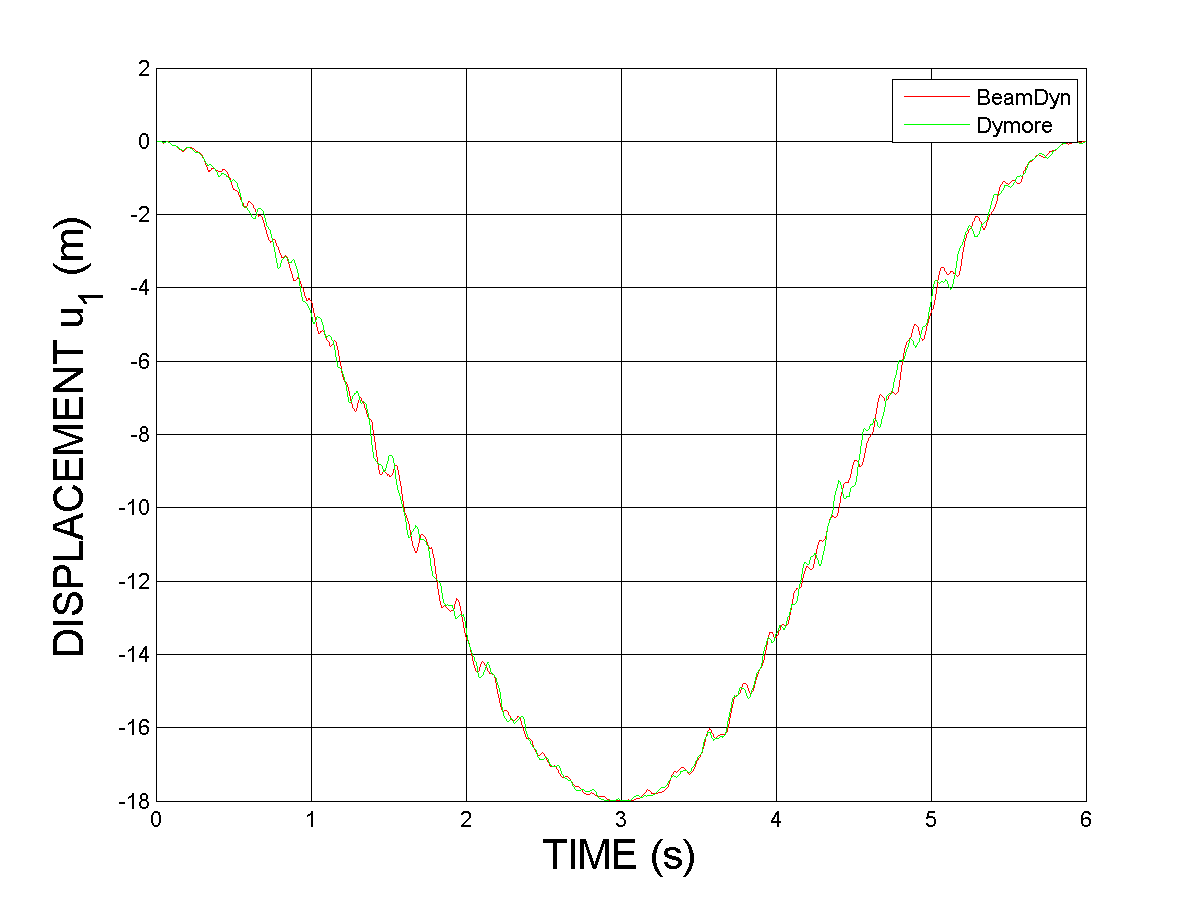
\includegraphics{figures/u1}}
			}			
		\subfigure[$u_2$]{
			\resizebox{3in}{!}{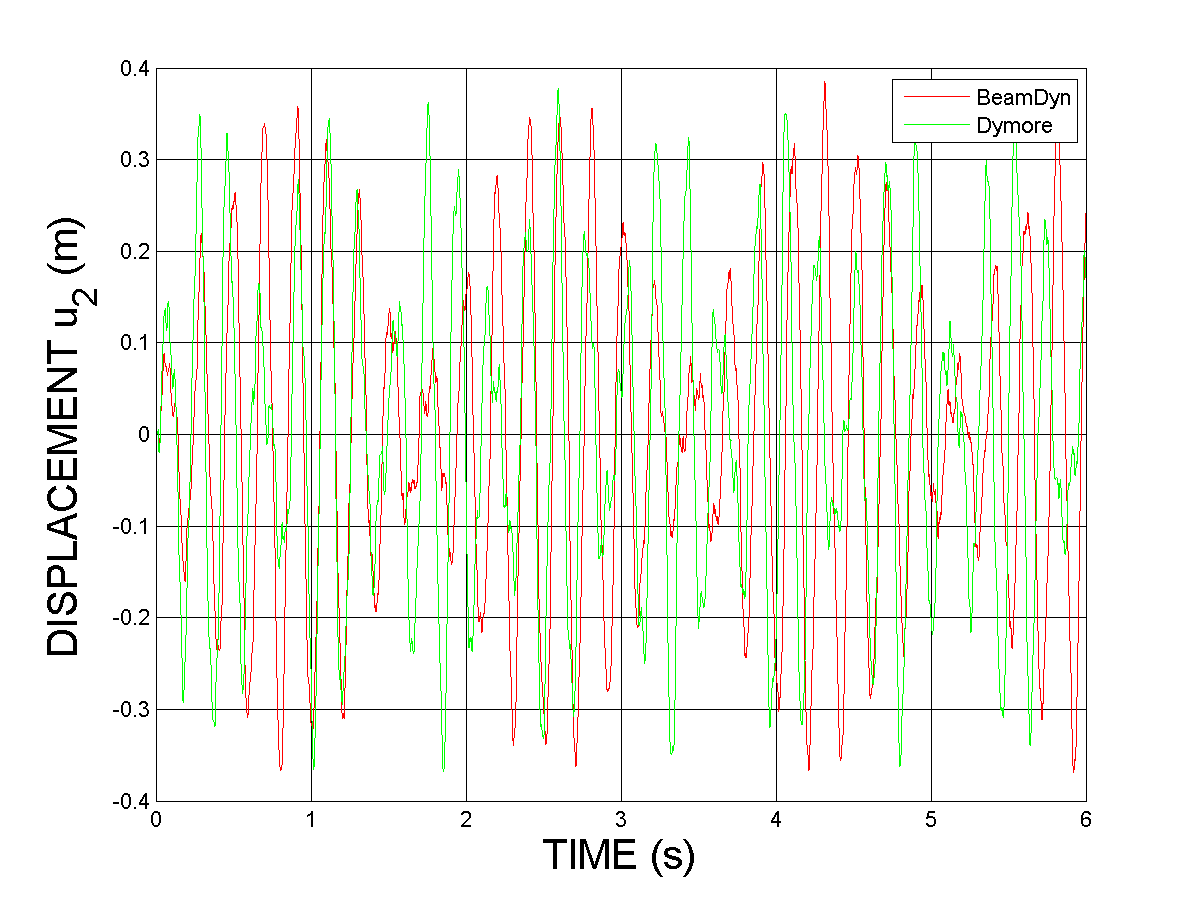
\includegraphics{figures/u2}}			
					}
					
		\subfigure[$u_3$]{
			\resizebox{3in}{!}{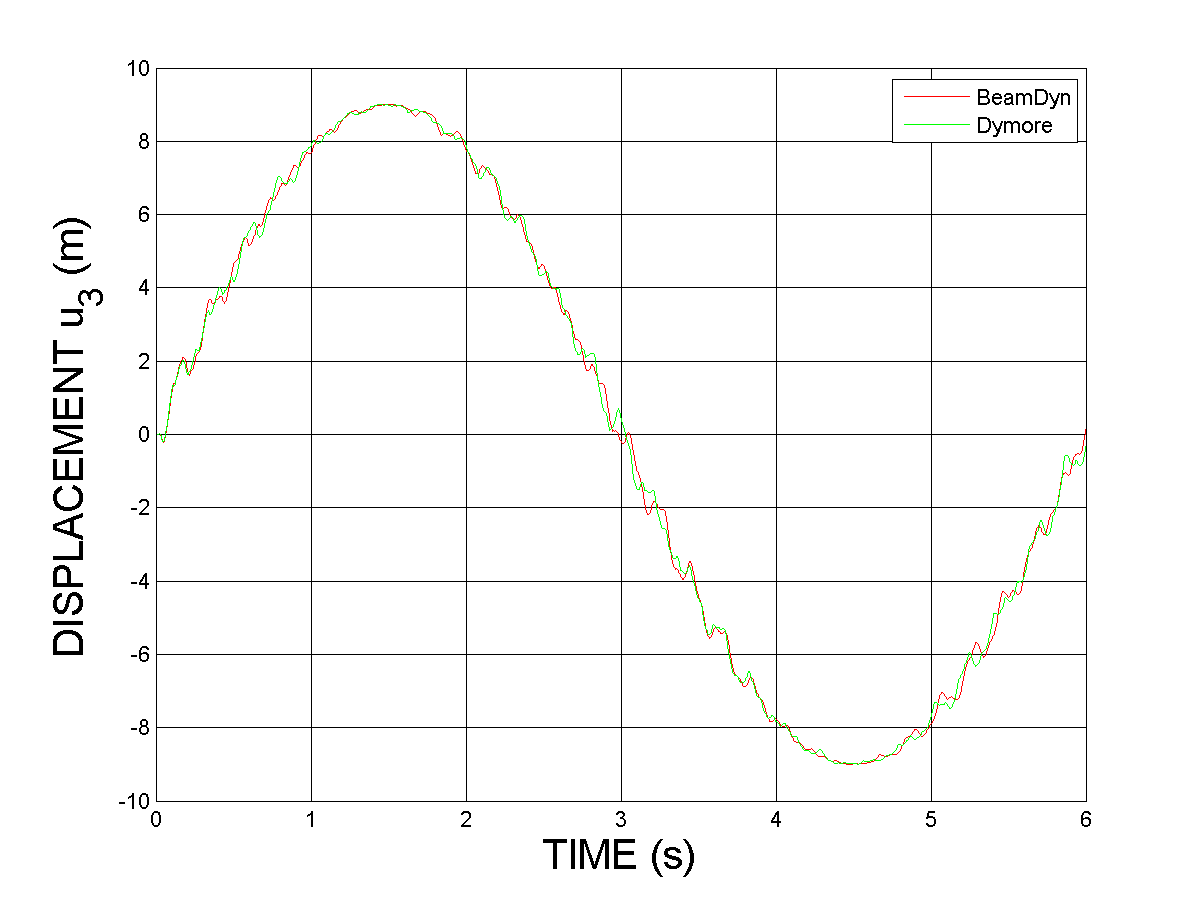
\includegraphics{figures/u3}}			
					}
		\subfigure[$p_1$]{
			\resizebox{3in}{!}{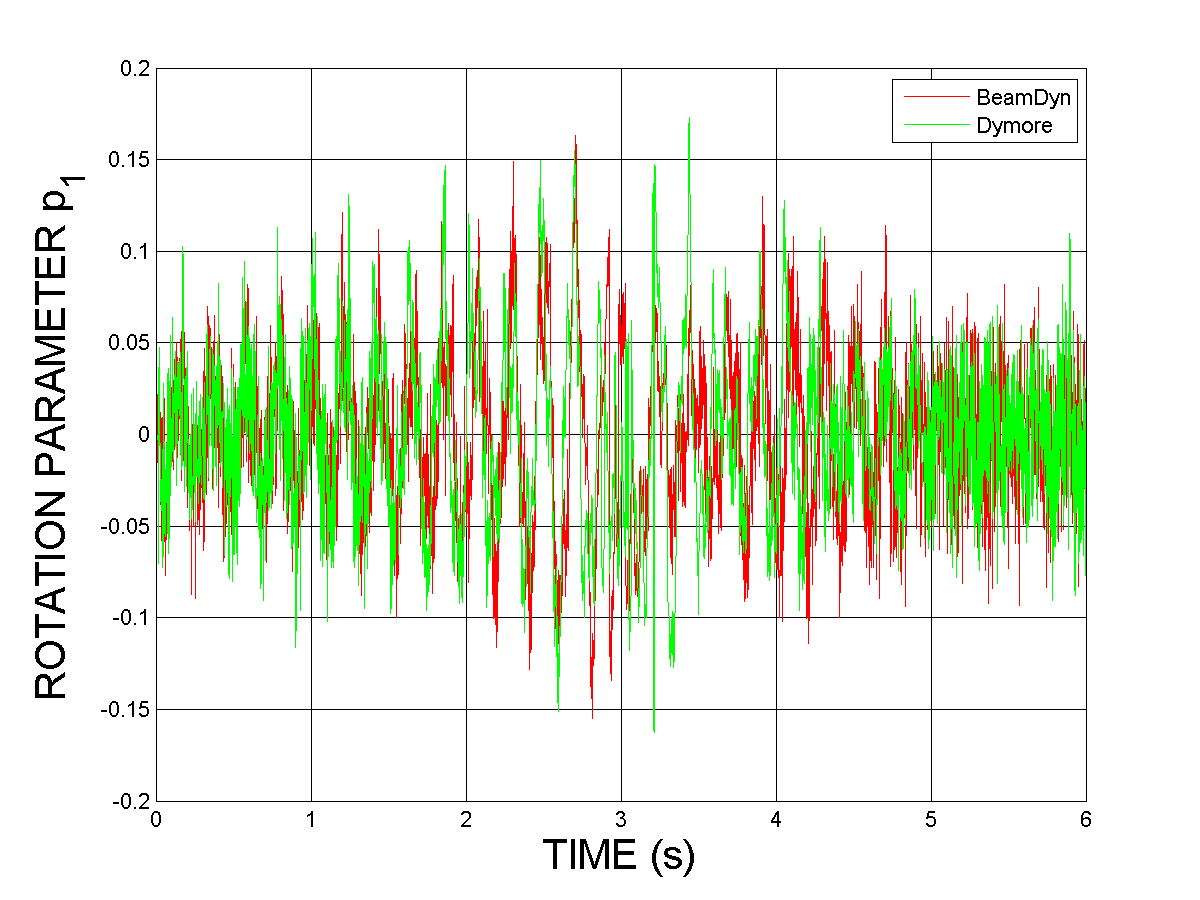
\includegraphics{figures/p1}}			
					}
					
		\subfigure[$p_2$]{
			\resizebox{3in}{!}{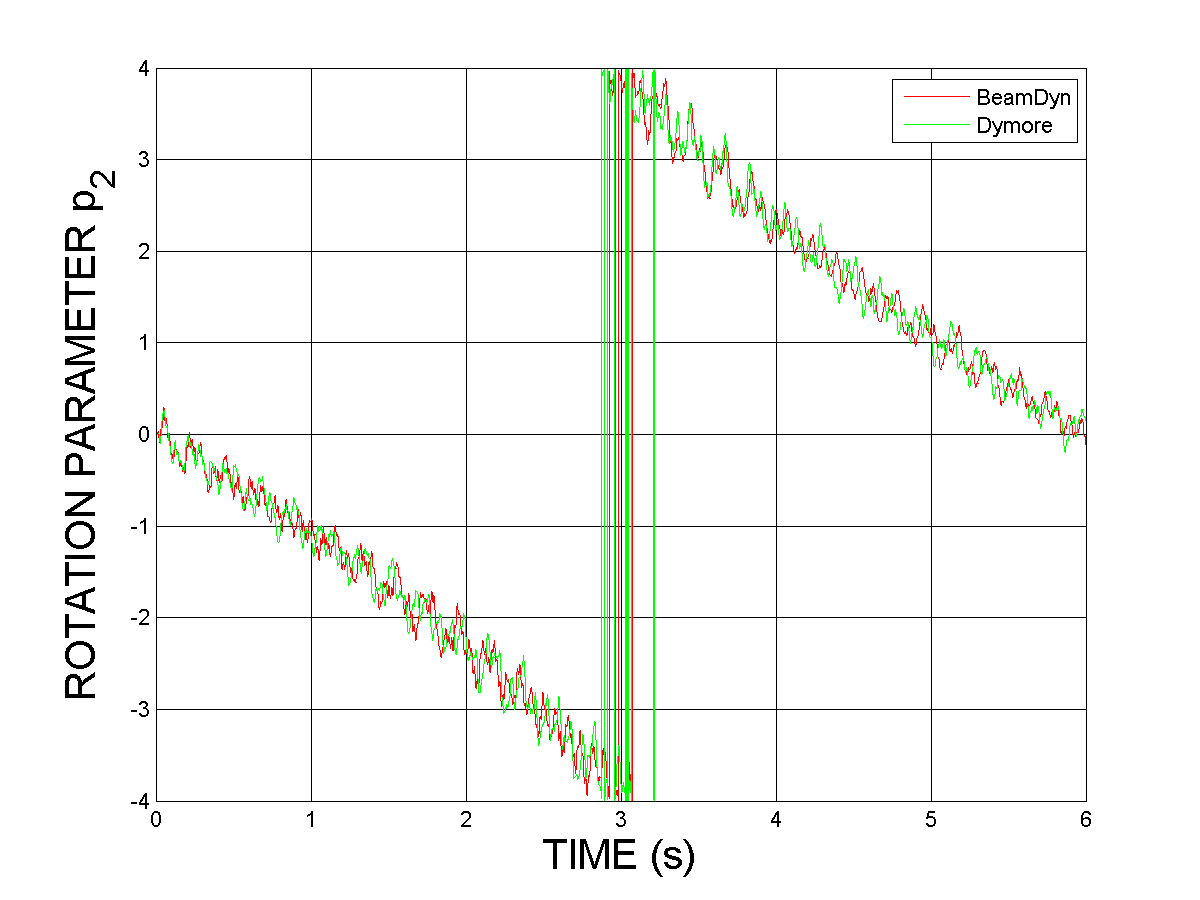
\includegraphics{figures/p2}}\label{fig:p2}			
					}
		\subfigure[$p_3$]{
			\resizebox{3in}{!}{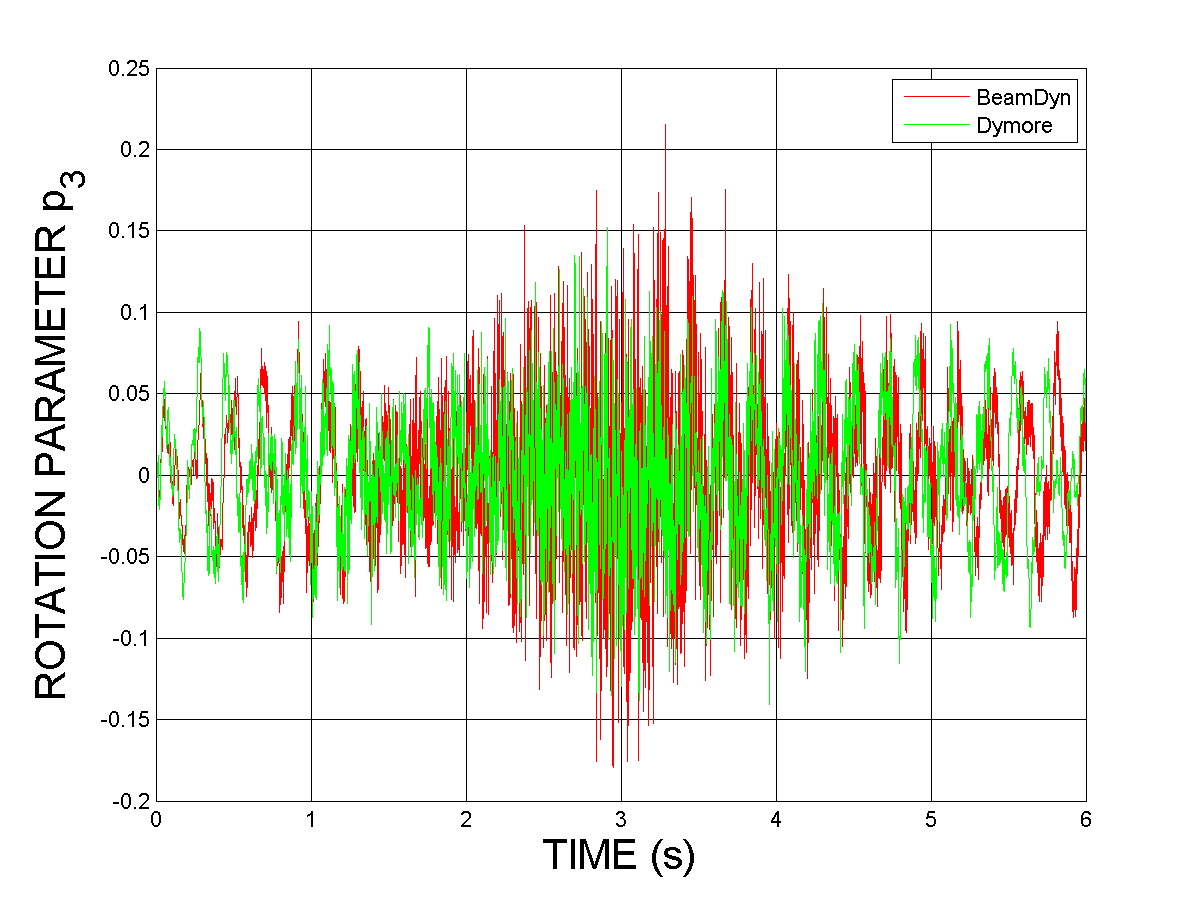
\includegraphics{figures/p3}}			
					}																
		% Normal caption:
		\caption{\label{fig:dym}Time history of $u_3$ for (a) no gravity load, and (b) gravity load }
	\end{center}
\end{figure}
It can be see in \ref{fig:p2} that a rescaling occurs halfway through the simulation as the rotation exceeds the $\pi$ rescaling limit. Since the time step is so small the numerical value of the rotation parameter is close to the singularity for multiple time step, thus triggering multiple rescaling operations.

\ref{fig:dynamic2} shows the root force for the no gravity load applied and gravity load applied cases. It can be seen that the root forces are higher for the case where the gravity force is applied, as expected.

\csmfigure{dynamic2}{figures/dynamic2}{5in}{Root force for dynamic simulation of BeamDyn with gravity load and without gravity load}

\newpage

\chapter{Conclusions and Future Work}
The objectives of this thesis were to systematically present the geometrically exact beam theory, present its finite element implementation in BeamDyn, and to detail verification and validation of BeamDyn. In the first chapter a review of prior work was completed to give an understanding of the current state of GEBT within the framework of the problem statement. Chapter two was devoted to mathematical and kinematic fundamentals that were necessary to the formulation of GEBT. In chapter three the VAM was presented which explained how the 3-D beam problem was split into a 2-D cross-sectional analysis and a 1-D beam analysis. Chapter four presented GEBT and spectral finite element method as implemented in BeamDyn. Chapter five explored a number of benchmark, numerical, and experimental examples that demonstrated the ability of BeamDyn to accurately analyze beam problems with: complex geometry, including initial curvature and initial twist; highly non-linear displacements; isotropic and anisotropic material properties; sharp gradients in material properties and its effect on spectral convergence; realistic wind turbine blades; and dynamic cases.

It was demonstrated in this thesis that BeamDyn is a rigorous tool for users wishing to analyze complex composite structures that may be approximated as beams. The application of spectral finite elements has further improved the performance of BeamDyn with respect to other tools based on GEBT for certain cases. It is unclear if the spectral FE approach improves the accuracy of realistic wind turbine blades with sharp gradients in the material properties. 

Future work in this area includes: further validation against utility scale dynamic wind turbine analysis; modal analysis; 3-D stress recovery; fully characterizing the effects of sharp gradients in material properties and geometry on spectral convergence; rigorous definition of shifting material properties for beams with initial curvature and twist; and fully coupling into the aeroelastic code FAST. Once this tool is coupled into FAST it will offer wind turbine designers a highly accurate alternative to full FEA packages such as ANSYS which have a high computational cost associated.
\end{document}